
\documentclass[a4paper]{article}

%Пакеты для математических символов:
\usepackage{amsmath} % американское математическое сообщество.
\usepackage{amssymb} % миллион разных значков и готический, ажурный шрифты.
\usepackage{amscd} % диаграммы, графики.
\usepackage{amsthm} % окружения теорем, определений и тд.
\usepackage{physics} % основные физические символы
%\usepackage{latexsym} % треугольники и пьяная стрелка.

%пакеты для шрифтов:
%\usepackage{euscript} % прописной шрифт с завитушками.
\usepackage{MnSymbol} % Значеки доказательства
\usepackage{verbatim} % улучшенный шрифт "пишущей машинки".
\usepackage{array} % более удобные таблицы.
%\usepackage{multirow} % мультистолбцы в таблицах.
%\usepackage{longtable} % таблицы на несколько страниц.
%\usepackage{latexsym}

\usepackage{etoolbox}
\usepackage{slashbox} %Разделениени текста \backslashbox{}{}
\usepackage{collectbox} % Добавляет коробочки, можно складывать туда текст)


\usepackage{hyperref} % Ссылки как внешние так и внутренние
\hypersetup{
    colorlinks=true,
    linkcolor=black,
    filecolor=magenta,      
    urlcolor=cyan,
    pdftitle={Overleaf Example},
    pdfpagemode=FullScreen,
    }
    
%Пакеты для оформления:
\RequirePackage[center, medium]{titlesec}% Стиль секций и заголовков
%\usepackage[x11names]{xcolor} % 317 новых цветов для текста.
\usepackage{float} % Позволяет использовать H, h! для локации фигур
%\usepackage{multicol} % набор текста в несколько колонн.
\usepackage{graphicx} % расширенные возможности вставки стандартных картинок.
\usepackage{subcaption} % возможность вставлять картинки в строчку
%\usepackage{caption} % возможность подавить нумерацию у caption.
\usepackage{wrapfig} % вставка картинок и таблиц, обтекаемых текстом.
\usepackage{cancel} % значки для сокращения дробей, упрощения, стремления.
\usepackage{misccorr} % в заголовках появляется точка, но при ссылке на них ее нет.
%\usepackage{indentfirst} % отступ у первой строки раздела
%\usepackage{showkeys} % показывает label формул над их номером.
%\usepackage{fancyhdr} % удобное создание верхних и нижних колонтитулов.
%\usepackage{titlesec} % еще одно создание верхних и нижних колонтитулов
\usepackage{hyperref} % Ссылки как внешние так и внутренние
\hypersetup{
    colorlinks=true,
    linkcolor=black,
    filecolor=magenta,      
    urlcolor=cyan,
    pdftitle={Overleaf Example},
    pdfpagemode=FullScreen,
    }
\usepackage{xcolor} %Позволяет перекрасить все страници
\definecolor{mycolor}{RGB}{244,228,215} %Цвет перекраски


%Пакеты шрифтов, кодировок. НЕ МЕНЯТЬ РАСПОЛОЖЕНИЕ.
\usepackage[utf8]{inputenc} % кодировка символов.
%\usepackage{mathtext} % позволяет использовать русские буквы в формулах. НЕСОВМЕСТИМО С tempora.
\usepackage[T1, T2A]{fontenc} % кодировка шрифта.
\usepackage[english, russian]{babel} % доступные языки.

%tikz:
\usepackage{tikz} % tikz
\usetikzlibrary{decorations.text} % позволяет делать текст вдоль кривой.
\usetikzlibrary{external} % позволяет кэшировать рисунки tikz.


\usepackage{pgfplotstable}

%Отступы и поля:
%размеры страницы А4 11.7x8.3in
\textwidth=7.3in % ширина текста
\textheight=10in % высота текста
\oddsidemargin=-0.5in % левый отступ(базовый 1дюйм + значение)
\topmargin=-0.5in % отступ сверху до колонтитула(базовый 1дюйм + значение)


%Сокращения
%Скобочки
\newcommand{\inrad}[1]{\left( #1 \right)}
\newcommand{\inner}[1]{\left( #1 \right)}
\newcommand{\infig}[1]{\left{ #1 \right}}
\newcommand{\insqr}[1]{\left[ #1 \right]}
\newcommand{\ave}[1]{\left\langle #1 \right\rangle}



%% Красивые <= и >=
\renewcommand{\geq}{\geqslant}
\renewcommand{\leq}{\leqslant}

%%Значек выполнятся
\newcommand{\per}{\hookrightarrow}

%%Векторная алгебра
\newcommand{\rot}{\text{rot}}
\renewcommand{\div}{\text{div}}
\renewcommand{\grad}{\text{grad}}

%% Более привычные греческие буквы
\renewcommand{\phi}{\varphi}
\renewcommand{\epsilon}{\varepsilon}
\newcommand{\eps}{\varepsilon}
\newcommand{\com}{\mathbb{C}}
\newcommand{\re}{\mathbb{R}}
\newcommand{\nat}{\mathbb{N}}
\newcommand{\stp}{$\filledmedtriangleleft$}
\newcommand{\enp}{$\filledmedsquare$}

%%Тензорный анализ ОТО теория поля
\newcommand{\Li}[1]{\mathfrak{L}_{#1}}
\newcommand{\crist}[3]{\cfrac{1}{2} \inner{g_{#1#2,#3} + g_{#1#3,#2} - g_{#2#3,#1}}}
\newcommand{\piv}[2]{\cfrac{\partial #1}{\partial #2}}

\makeatletter
\newcommand{\sqbox}{%
    \collectbox{%
        \@tempdima=\dimexpr\width-\totalheight\relax
        \ifdim\@tempdima<\z@
            \fbox{\hbox{\hspace{-.5\@tempdima}\BOXCONTENT\hspace{-.5\@tempdima}}}%
        \else
            \ht\collectedbox=\dimexpr\ht\collectedbox+.5\@tempdima\relax
            \dp\collectedbox=\dimexpr\dp\collectedbox+.5\@tempdima\relax
            \fbox{\BOXCONTENT}%
        \fi
    }%
}
\makeatother
\newcommand{\mergelines}[2]{
\begin{tabular}{llp{.5\textwidth}}
#1 \\ #2
\end{tabular}
}
\newcommand\tab[1][0.51cm]{\hspace*{#1}}
\newcommand\difh[2]{\frac{\partial #1}{\partial #2}}
\newcommand{\messageforpeople}[1]{HSE Faculty of Physics \ \ HSE Faculty of Physics HSE Faculty of Physics \ \ HSE Faculty of Physics HSE Faculty of Physics \ \ HSE Faculty of Physics HSE Faculty of Physics \ \ HSE Faculty of Physics HSE Faculty of Physics \ \ HSE Faculty of Physics HSE Faculty of Physics \ \ HSE Faculty of Physics HSE Faculty of Physics \ \ HSE Faculty of Physics HSE Faculty of Physics \ \ HSE Faculty of Physics }


\numberwithin{equation}{section}

\begin{document}


% \pagecolor{mycolor}
\pagestyle{empty}
\oddsidemargin=-1.18in
\topmargin=-1.5in

\begin{titlepage}
\begin{tikzpicture}
    \draw [white] (0, 0) ellipse (4.1in and 5.7in);
    \path [postaction={
    decoration={text along path,
    text={\messageforpeople{}},
    text align=center,
    raise=0mm,
    reverse path}, decorate}]
    [postaction={
    decoration={text along path,
    text={\messageforpeople{}},
    text align=center,
    raise=3mm,
    reverse path}, decorate}]
    [postaction={
    decoration={text along path,
    text={\messageforpeople{}},
    text align=center,
    raise=6mm,
    reverse path}, decorate}]
    [postaction={
    decoration={text along path,
    text={\messageforpeople{}},
    text align=center,
    raise=9mm,
    reverse path}, decorate}]
    [postaction={
    decoration={text along path,
    text={\messageforpeople{}},
    text align=center,
    raise=12mm,
    reverse path}, decorate}] 
    [postaction={
    decoration={text along path,
    text={\messageforpeople{}},
    text align=center,
    raise=15mm,
    reverse path}, decorate}]
    [postaction={
    decoration={text along path,
    text={\messageforpeople{}},
    text align=center,
    raise=18mm,
    reverse path}, decorate}]
    [postaction={
    decoration={text along path,
    text={\messageforpeople{}},
    text align=center,
    raise=21mm,
    reverse path}, decorate}] 
    [postaction={
    decoration={text along path,
    text={\messageforpeople{}},
    text align=center,
    raise=24mm,
    reverse path}, decorate}]
    [postaction={
    decoration={text along path,
    text={\messageforpeople{}},
    text align=center,
    raise=27mm,
    reverse path}, decorate}]
    [postaction={
    decoration={text along path,
    text={\messageforpeople{}},
    text align=center,
    raise=30mm,
    reverse path}, decorate}] 
    [postaction={
    decoration={text along path,
    text={\messageforpeople{}},
    text align=center,
    raise=33mm,
    reverse path}, decorate}]
    [postaction={
    decoration={text along path,
    text={\messageforpeople{}},
    text align=center,
    raise=36mm,
    reverse path}, decorate}]
    [postaction={
    decoration={text along path,
    text={\messageforpeople{}},
    text align=center,
    raise=39mm,
    reverse path}, decorate}] 
    [postaction={
    decoration={text along path,
    text={\messageforpeople{}},
    text align=center,
    raise=42mm,
    reverse path}, decorate}]
    [postaction={
    decoration={text along path,
    text={\messageforpeople{}},
    text align=center,
    raise=45mm,
    reverse path}, decorate}]
    [postaction={
    decoration={text along path,
    text={\messageforpeople{}},
    text align=center,
    raise=48mm,
    reverse path}, decorate}] 
    [postaction={
    decoration={text along path,
    text={\messageforpeople{}},
    text align=center,
    raise=51mm,
    reverse path}, decorate}]
    [postaction={
    decoration={text along path,
    text={\messageforpeople{}},
    text align=center,
    raise=54mm,
    reverse path}, decorate}]
    [postaction={
    decoration={text along path,
    text={\messageforpeople{}},
    text align=center,
    raise=57mm,
    reverse path}, decorate}] 
    [postaction={
    decoration={text along path,
    text={\messageforpeople{}},
    text align=center,
    raise=60mm,
    reverse path}, decorate}]
    [postaction={
    decoration={text along path,
    text={\messageforpeople{}},
    text align=center,
    raise=63mm,
    reverse path}, decorate}]
    [postaction={
    decoration={text along path,
    text={\messageforpeople{}},
    text align=center,
    raise=66mm,
    reverse path}, decorate}] 
    [postaction={
    decoration={text along path,
    text={\messageforpeople{}},
    text align=center,
    raise=69mm,
    reverse path}, decorate}]
    [postaction={
    decoration={text along path,
    text={\messageforpeople{}},
    text align=center,
    raise=72mm,
    reverse path}, decorate}]
    (0, 0) ellipse (2.75in and 4.96in);
    \node at (0, 3.2in) {\Large\textbf{Домашняя работа 1}};
    \node at (0, 0in) {
\includegraphics[height=4in]{FOPF.png}};
    \node at (0, -3in) {Авторы:};
    \node at (0, -3.2in) {Карибджанов Матвей};
    \node at (0, -3.5in) {2023};
\end{tikzpicture}

%2.75in and 4.96in
\end{titlepage}

\oddsidemargin=-0.5in
\topmargin=-0.5in
\pagestyle{plain}

\newpage
\tableofcontents
\newpagestyle{main}{
\setfootrule{0.4pt}
\setfoot{}{\thepage}{\sectiontitle }}
\pagestyle{main}



\section{Ведение}

Рассмтрим гуппу симметрий тетраидера $T_d$. Легко понять что количество элентов этой 
группы это $3\dot 4 \dot 2 = 24$. 3 это количество повротов вокруг вершины,
4 так как все 4 вершины эквиваленты умножаю на 2 так как уичитывам так же отражения.

\section{Поиск элементов}

\subsection{Повороты на $0 \land \ \cfrac{\pi}{3} \land \ \cfrac{2 \pi}{3}$}

Сначала найдем чевидные элемнты группы это повороты на 
$0 \land \ \cfrac{\pi}{3} \land \ \cfrac{2 \pi}{3}$ вогруг осей проходящих через 
высоту падающай из произвольной вершины. Таик такую группу 
повротов мы уже знаем это $C_3^n$ приэтом заметим что для любой вершины 
еденичные элемнты будут совпадть поэтому всего повротов будет $4*3 = 8$. 
Еслри пронумеровать вершины то можем обозначить элемнты ледующим обзазам

\begin{eqnarray}
    C_3^{n \ v}, \ n \in \insqr{1, 2}, \ v \in \insqr{0, 1, 3, 4}
\end{eqnarray}

\begin{figure}[H]
    \centering
    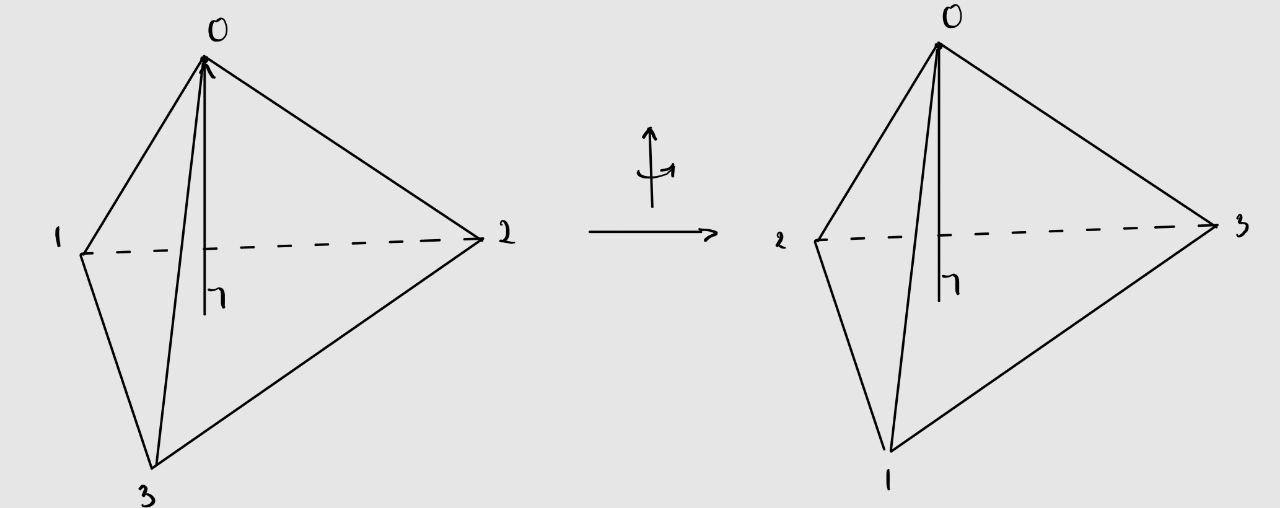
\includegraphics[width=0.5\linewidth]{su/C_10_3.jpg}
    \caption{Действие элемента $C^{1 \ 0}_{3}$}
\end{figure}

\subsection{Повороты на $\pi$}

Такжем можем легко заметить что есть повороты на $\pi$ вокруг оси соединяющей
середины противоположных ребер. Тоесть для всего таких элементов $6/2 = 3$, 
делю на 2 тк для ребрер $e_1 e_2$ и $e_2 e_1$ один и тот же.  Обозначим их так:

\begin{equation}
    C_{2}^{e_1 \ e_2} = C_{2}^{e_2 \ e_1} = C_{2}^{e_1} , \ e_1, e_2 \in \inner{01, 02, 03, 12, 13, 23}
\end{equation}

\begin{figure}[H]
    \centering
    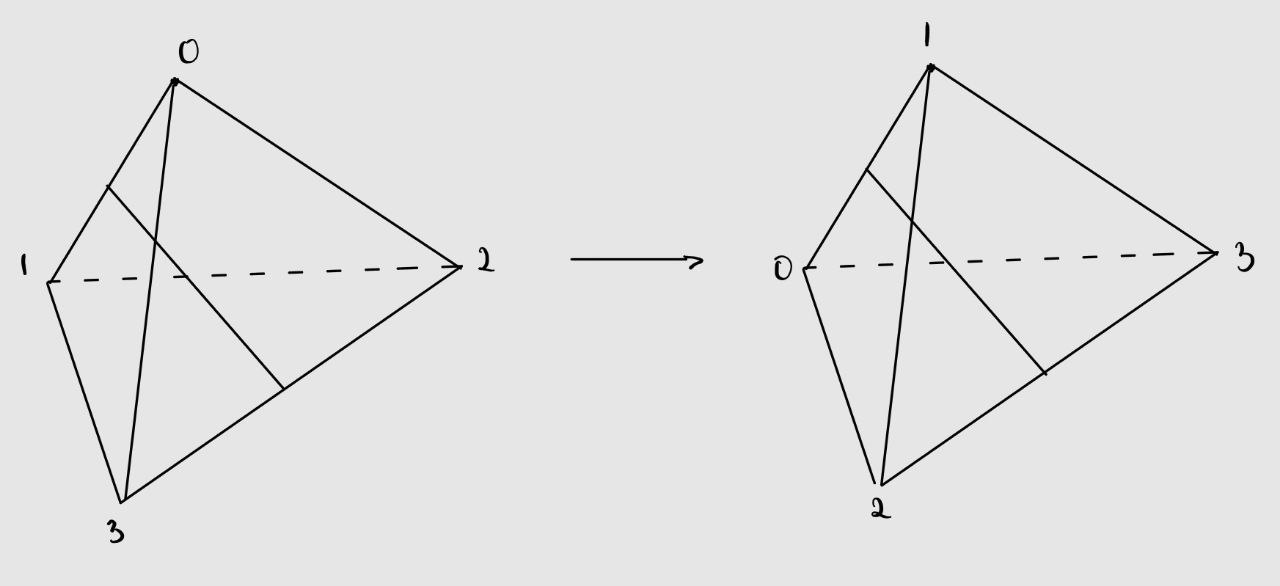
\includegraphics[width=0.5\linewidth]{su/C_15_2.jpg}
    \caption{Действие элемента $C^{01}_{2}$}
\end{figure}

\subsection{Отражения}

И самое последнее, что можно легко зметить это отраженияо тносительно плоскости 
оразуемой ребром и серединой протипротоволежащего ребра. Таким образом всего 
элементов будет $6$ - количество ребер. Введем следующее обозначения:

\begin{equation}
    \sigma^{e_1}, e_1 \in \inner{01, 02, 03, 12, 13, 23}
\end{equation}

\begin{figure}[H]
    \centering
    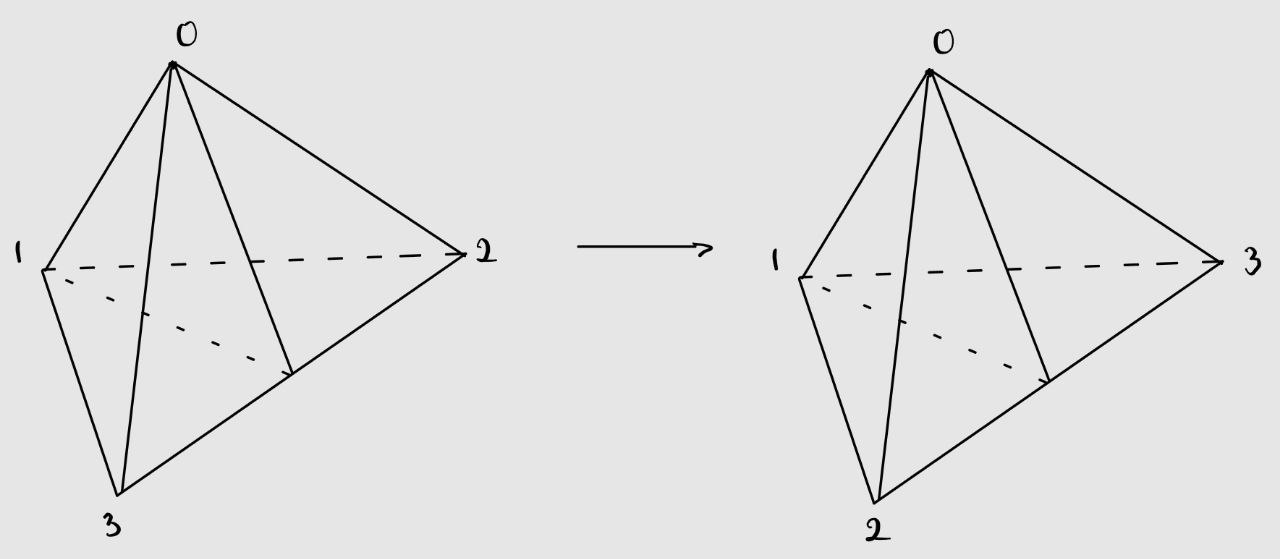
\includegraphics[width=0.5\linewidth]{su/sigma_01.jpg}
    \caption{Действие элемента $\sigma^{01}$}
\end{figure}

\subsection{Дополнение до группы}
Как можно заметить пака что элементов меньше чем требуется, поэтому пред оставлю 
машине посчитаь за меня оставшиеся элементы. Но перед этим я зметил что
группу сииметрий тетраидера и вроде как любой фигуры (для тетраидера и 3Д 
фигур точно работает), можно задать изоморфизм на подгуппу кос (без учета 
нахлеста) с количеством нитей равным количеству вершин фигуры. 
Тоесть можем перписать наши эленты следующи образом:

\begin{eqnarray}
    e &\to &0123\\
    C_3^{1 \ 0} &\to & 0231 \\
    C_2^{01} &\to & 1032\\
    \sigma^{01} &\to & 0132
\end{eqnarray}

Думаю изорфизм остальных элементов очевиден. Следствем такого изоморфизма 
является тот факт, что моя группа э то Гуппа престановок 4 элемнтов $\inner{S_4}$
Тут же заметим простой факт элементы из $C_3$ это циклическая перстановка 3 элементов, $C_2$ - перстановка 
элентов внутри 2х пар, $\sigma$ перестановка элемнтов внутри одной пары. 
Можно леко дополнить группу протой найдя оставшиеся перстаовки,
но я написал код так, что омотри код.

В итоге получу полную группу $T_d=$ (0123, 1032, 2301, 3210, 0231, 
0312, 2130, 3102, 1320, 3021, 1203, 2013, 0132, 0321, 0213, 3120, 2103, 
1023, 1230, 1302, 2031, 3012, 2310, 3201)


\section{Таблица Келли}
А таблица Келли для сответствующего порядка элементов группы

\begin{table}[H]
    \centering
    \pgfplotstabletypeset[precision=0,
       col sep=space]{su/kelli.csv}
\end{table}

\section{Поиcк представлений}

\subsection{Классы сопряженности}

С помощью простого перебора программой я получил следующий классы:

\begin{eqnarray}
    0123\\
    2301, 3210, 1032\\
    1203, 2130, 0231, 3102, 1320, 3021, 2013, 0312\\
    0132, 1023, 0321, 0213, 2103, 3120\\
    1230, 3201, 2031, 1302, 3012, 2310
\end{eqnarray}

\subsection{Анализ результатов классов смежности}

Сначала перепишем классы в дркгом виде для простоты объяснения:

\begin{eqnarray}
    e\\e
    C^{01}_2, C^{03}_2, C^{02}_2\\
    C^{21}_3, C^{10}_3, C^{13}_3, C^{20}_3, C^{12}_3, C^{11}_3, C^{22}_3, C^{23}_3\\
    s^{13}, s^{01}, s^{12}, s^{23}, s^{03}, s^{02}\\
    C^{02}_2*s^{23}, C^{02}_2*s^{01}, C^{01}_2*s^{12}, C^{01}_2*s^{03}, C^{01}_2*s^{02}, C^{01}_2*s^{13}
\end{eqnarray}

Как мы видим из не привиалных классов у нас есть 2 Нормальные подгрууппы поворотов
на $\pi$ и $\cfrac{2\pi}{3}$ соттветственно. Так же есть подгуппа отражений
и произведение отражений и повротов на $\pi$.

Как мы знаем всегда есть одно тривиаольное одномерное преодставление.
Но есть одно знако переменно порожденной не однозначностью выбора опредлителя
при поворотах, я могу с уверенность сказсть это так как группа повротов 
тераидера являтся подгуппой симмтрий шара тоесть группы $SO(3)$:


\begin{tabular}[pos]{c|c|c|c|c|c}
            & $e$ & $C_2$   & $C_3$ & $\sigma$  & $\sigma*C_2$  \\ \hline
    $A_1$   & $1$ & $1$     & $1$   & $1$       & $1$           \\ \hline
    $A_2$   & $1$ & $1$     & $1$   & $-1$      & $-1$          
\end{tabular}

Дальше пользуясь соотношением 
\begin{equation}
    C = \sum_i s^2_i = 1 + 1 + s^2_3 + s^2_4 + s^2_5
\end{equation}

Можем нати что оставшиеся 3 предсталения имеют следующие размерности 
$s_3 = s_4 = 3, \ s_5 = 2$. Можно было и рантше воспользоваться этим 
соотношениеим и порлучить, что всего есть 2 одномерных представления.

\subsection*{3-х Мерные представления}

Трех мреные мы всегда хорошо занаем так как у нас группа симмтрий 
тетраидера составленная из повротов и отражений, то матричные представления 
это повроты вокруг некотрых осей  матри поврота всегда можно передставить 
в виде:

\begin{gather}
    \begin{pmatrix}
        \cos \phi & \sin \phi & 0 \\
        \sin \phi & \cos \phi & 0 \\
        0 & 0 & \pm 1 
    \end{pmatrix}
\end{gather}

Как и в пршлый раз два предсталения это следствие не однозначности выбора 
определителя.

Получим характеры $\pm 1 + 2 \cos \phi$

\begin{tabular}[pos]{c|c|c|c|c|c}
        & $e$   & $C_2$ & $C_3$ & $\sigma$  & $\sigma*C_2$  \\ \hline
$A_1$   & $1$   & $1$   & $1$   & $1$       & $1$           \\ \hline
$A_2$   & $1$   & $1$   & $1$   & $-1$      & $-1$          \\ \hline
$T_1$   & $3$   & $-1$  & $0$   & $-1$      & $1$           \\ \hline
$T_2$   & $3$   & $-1$  & $0$   & $1$       & $-1$          
\end{tabular}

Для первых двух классов расчет одинкаов там $+1$:
\begin{eqnarray}
    e: \ 1 + 2 \cos \phi \ \vline_{\phi = 0} = 1 + 2 = 3 \\
    C_2: \ 1 + 2 \cos \phi \ \vline_{\phi = \pi} = 1 - 2 = -1 \\
    C_3: \ 1 + 2 \cos \phi \ \vline_{\phi = \cfrac{2 \pi}{3}} = 1 - 2 \cdot \cfrac{1}{2} = 0
\end{eqnarray}

Для последнийх двух столбцов отличие в знаке перед единицей, как в одномерных представленийх
собственно это они и есть толко записанные как блок трех мерной матрици.


\begin{eqnarray*}
    \sigma: \pm 1 \mp 2 \cos \phi \ \vline_{\phi = 0} = \pm 1 \mp 2 = \mp 1 \\
    \sigma * C_2: \mp 1 \pm \cos \phi \ \vline_{\phi = 0} = \pm 1
\end{eqnarray*}

\subsection{Двумерное представлене и таблица харектеров}

Последнюю строку для двумерного представления найдем из 
соотношения ортгональности.

\begin{gather}
    \begin{pmatrix}
        1 & 1 & 3 & 3 & 2
    \end{pmatrix}
    \begin{pmatrix}
        1 \\ 1 \\ -1 \\ -1 \\ x
    \end{pmatrix}
    = 1 + 1 - 3 - 3 + 2x = 0
    \implies 
    x = 2
\end{gather}


\begin{gather}
    \begin{pmatrix}
        1 & 1 & 0 & 0 & x    
    \end{pmatrix}
    \begin{pmatrix}
        1 \\ 1 \\ -1 \\ -1 \\ 2
    \end{pmatrix}
    = 1 + 1 + 2x = 0
    \implies 
    x = -1
\end{gather}

и так далее. В итоге получим:

\begin{tabular}[pos]{c|c|c|c|c|c}
    & $e$   & $C_2$ & $C_3$ & $\sigma$  & $\sigma*C_2$  \\ \hline
$A_1$   & $1$   & $1$   & $1$   & $1$       & $1$           \\ \hline
$A_2$   & $1$   & $1$   & $1$   & $-1$      & $-1$          \\ \hline
$T_1$   & $3$   & $-1$  & $0$   & $-1$      & $1$           \\ \hline
$T_2$   & $3$   & $-1$  & $0$   & $1$       & $-1$          \\ \hline
$E$     & $2$   & $2$   & $-1$  & $0$       & $0$          
\end{tabular}



\section{Преобразование функций}

\subsection{Одномерные пердставления}

Здесь мне повезло тетраидер очень хорошая фигура и если выбирать любой 
базис то в нем все оси равновыделенны, это мы знаем еще с аналитической
механики, когда расчитывали моенты инерции тетраидера, поэтому не 
побоюсь этим воспользоваться.

Для начала очевидное представление $A_1$ так как оно единичное то 
а повороты происходят в различых осях то сответственно только $x^2+y^2+z^2$.

\subsection{Трехмерные передставления}

Явно я знаю только одно представление, это 4-мерное, при этом оно приводимо.
Выглядят преобразования следующим образом:
\begin{gather}
    D(1032)=
    \begin{pmatrix}
        0& 1& 0& 0\\
        1& 0& 0& 0\\
        0& 0& 0& 1\\
        0& 0& 1& 0\\
    \end{pmatrix}
    \in C_2, \
    D(1203)=
    \begin{pmatrix}
        0& 1& 0& 0\\
        0& 0& 1& 0\\
        1& 0& 0& 0\\
        0& 0& 0& 1\\
    \end{pmatrix}
    \in C_3, \
    D(0132)=
    \begin{pmatrix}
        1& 0& 0& 0\\
        0& 1& 0& 0\\
        0& 0& 0& 1\\
        0& 0& 1& 0\\
    \end{pmatrix}
    \in \sigma
\end{gather}
Можно по анологии построить остальные матрицы представления. Такие матрицы дейтвуют на пространстве
функций:
\begin{gather}
    \begin{pmatrix}
        0& 1& 0& 0\\
        0& 0& 1& 0\\
        1& 0& 0& 0\\
        0& 0& 0& 1\\
    \end{pmatrix}
    \begin{pmatrix}
        a\\ b\\ c\\ f
    \end{pmatrix}
    =
    \begin{pmatrix}
        a\\ b\\ c\\ f
    \end{pmatrix}
\end{gather}

Найдем такую матрицу что будет преобразовывть мои $D(g)$ в:

\begin{gather}
    S^{-1} D(g) S =
    \begin{pmatrix}
        A& C\\
        0& B
    \end{pmatrix};
    \ B = 3\times 3, \  A = 1 \times 1, \ C = 1 \times 3
\end{gather}

Тут позволю себе отойти от темы. Я говрил вам на паре что матрица
иваритного подпространства не всегда должна иметь $C = 0$. Явно это можно увидеть 
из следующих сображений.

\begin{gather}
    \begin{pmatrix}
        A& C\\
        0& B
    \end{pmatrix}
    \begin{pmatrix}
        x_1\\ x_2
    \end{pmatrix}
    =
    \begin{pmatrix}
        A x_1 + B x_2\\ B x_2
    \end{pmatrix}
\end{gather}

То есть $x_2$ ивариантное подпространство. Я счтаю то это тот самы случай когда
это важно, потому что если бы я искал $C = 0$ то боюсь что не нашел бы такого пердставления.

Возварыюсь к теме, иными словами я должен сотавит из функций $(a, b, c, f)$ 4
линейных комбинации котрые будут удовлетворять:

1. 3 из них переходят сами в себя при действии любого элента группы

2. 4 должны сотвлять полный базис в протранстве 4-х элментов

3. 3 из первого пункта при перестановке двух элементов любых 
элементов и циклической должны выржать ся друг через друга так что-бы
при не возникало линеных компбинвций этих любых двух функций.

1 - требование ивариантности трех мерного пространства.

2 - требование не вырожденности преобразований.

3 - требование позволит обозначить эти три линейные комбинации за $x, y, z$
и тогда при перобразованих будет происходить например следующее $B (x, y, z) = (\alpha z, \beta x, \gamma z)$.
Кароче говря мы найдем самый трех мерный базис функций. Но может возникнуть вопрос почему я говорю
только о одной циклической перестановке и престановке двух элементов, на самом деле этих двух действий 
достаточно чтобы потсроить любое другое действие группы.

Матрицу $S$ я угадал но надо сказть что она более менее тривильна:

\begin{gather}
    S = 
    \begin{pmatrix}
        1& -1& -1& 1\\
        1& 1& -1& -1\\
        1& -1& 1& -1\\
        1& 0& 0& 0
    \end{pmatrix}
\end{gather}

То-есть функции ы новом базисе
\begin{gather}
    \begin{pmatrix}
        a - b - c + f\\ a + b - c - f\\ a - b + c - f\\ a
    \end{pmatrix}
    ; \
    \begin{pmatrix}
        x\\ y\\ z
    \end{pmatrix}
    =
    \begin{pmatrix}
        a - b - c + f\\ a + b - c - f\\ a - b + c - f
    \end{pmatrix}
\end{gather}


Проверка 2-огг условия происходят явно, $det(S) \neq 0$. Проверку 3 условия я не знаю как делать в общем случае,
но ее можно сделать явно по перемножать матрици:

\begin{gather}
    S^{-1}D(1032)S = 
    \cfrac{1}{2} 
    \begin{pmatrix}
        2& 2& -2& -2\\
        0& 4& -2& -2\\
        0& 3& -3& -1\\
        0& 3& -1& -3
    \end{pmatrix}
\end{gather}
\begin{gather}
    S^{-1}D(1203)S = 
    \begin{pmatrix}
        1& 0& 0& 0\\
        0& 0& 1& 0\\
        0& 0& 0& 1\\
        0& 1& 0& 0
    \end{pmatrix}
\end{gather}
\begin{gather}
    S^{-1}D(0132)S =
    \cfrac{1}{2}
    \begin{pmatrix}
        2& -2& 2& -2\\
        0& -1& 3& -3\\
        0& -2& 4& -2\\
        0& -3& 3& -1
    \end{pmatrix}
\end{gather}

С остальными аналогично. Для 3 тоже можно проверит явно $D(1032) (a - b - c + f) = -(a - b + c - f) $ или 
$D(0132)(a - b + c - f) = (a - b - c + f)$ или $D(1203)(a - b + c - f) = (a + b - c - f)$ и так далее.

Дальше так же протсо можно понять, что трех мерное представление $T_2$ в трех мерном 
пространстве будет преобразовывать $(x, y, z)$ или для квадратичных функций
$(xy, xz, yz)$. Возможен вопрос почему не $T_1$ рассмтрим $\sigma$, обычно 
отражение преводит $z \to -z$ поэтому рассмтрев обратный элемент $T_2^{-1}(\sigma) z \to -z$.

\subsection{Двумерное предствление}

Пля двумерного представления все сложнее. Надо выбрать какойто ортогональный 
базис но прижтом сохранить равновыделенност каждой оси. Понятно что для линейных
функций такого базиса не сыщешь, а вот для квдратичных функций можно. Еще 
надо заметить две вещи, первая я немного соврал когда говорил что все оси
равно выделенны на самомделе это немного не так, если мы можем повренуть тетраидер
и так что одна грань будет лежать например в $(Ox, Oy)$ и тогда у нас $x, y$
будет выделенной плоскостью. Второе, что мне нужно подметить так это, очевидно
что вумерное представлени берется из факторизации трехмерного на два одмнорных
и однодвумерное. Поэтому надо выбрать такой базис котрый будет ортогонален
$x^2 + y^2 + z^2$. И такой я знаю например $(x^2 - y^2, z^2 - \cfrac{1}{2} (x^2 + y^2))$ 







\end{document}